\chapter{Dívida Técnica}
\label{cap:cap2}

Neste capítulo, descrevemos o que é uma dívida técnica, seus principais tipos e formas de classificação juntamente com as atuais abordagens de gerenciamento.


\section{Introdução}


Desenvolver software é uma atividade complexa por diversas razões. Entre elas estão as dificuldades em gerenciar requisitos muitas vezes ambíguos e até mesmo conflitantes, a imprevisibilidade do contexto no qual o software está inserido e as particularidades das tecnologias utilizadas. Nem sempre todos esses fatores poderão ser devidamente tratados nos projetos de software. Em algumas circunstâncias, pode não ser possível lidar com todos eles de forma satisfatória devido ao seu número excessivo e a falta de recursos disponíveis tais como a quantidade de membros na equipe e o tempo disponível para realizar as tarefas. Essa falta de recursos pode fazer com que seja necessário realizar algumas escolhas para que um projeto possa ser viabilizado. Existem algumas opções para tornar viável um projeto que tenha recursos incompatíveis.  A solução mais óbvia é conseguir mais recursos. Outra opção é a eliminação ou simplificação  de determinadas funcionalidades e com isso diminuir o esforço necessário para realizar o projeto.   Naturalmente, nem sempre é possível que uma dessas duas opções possa ser seguida. Isso pode levar a uma situação onde algumas das atividades do projeto tenham de ser realizadas utilizando menos recursos. Essa redução nos recursos necessários pode ser alcançada melhorando a eficiência dos processos ou diminuindo a qualidade no qual eles são realizados. Um aperfeiçoamento na eficiência dos processos é algo que, apesar de positivo, pode não ser alcançável. Enquanto isso, quase sempre é possível diminuir a qualidade no qual um processo é realizado. Isso faz com que essa diminuição na qualidade seja a solução mais fácil para resolver o problema da falta de recursos. Uma dívida técnica é a diminuição na qualidade de algum aspecto do projeto de software para viabilizá-lo e que gerará dificuldades adicionais para  desenvolvê-lo no futuro.

Uma das formas de definir uma dívida técnica é como \textbf{algo} no software ou no seu processo de desenvolvimento que não está ideal e que por causa disso poderá haver algum tipo de \textbf{dificuldade adicional}. Esse \textbf{algo} pode ser a existência de código de má qualidade, um design inadequado, uma tecnologia ultrapassada dentro outros. A \textbf{dificuldade adicional} é o aumento de esforço necessário para realizar alguma atividade relacionada ao software no futuro.  Esse aumento de esforço não existiria caso o \textbf{algo} também não existisse. Essa é uma definição propositalmente ambígua já que o termo dívida técnica foi demasiadamente estendido e aplicado em diversas situações tornando desafiadora a tarefa de defini-lo precisamente. 



Para ilustrarmos o que é uma dívida técnica forneceremos alguns exemplos. O primeiro deles é baseado no código da Figura \ref{fig:cap1_exemplo_divida_codigo}. Nele, há um trecho de uma classe chamada RelatorioV1. Essa classe tem a função de receber os nomes e endereços de algumas pessoas e gerar um relatório em algum formato previamente estabelecido. A função adicionarLinha é acionada por outras classes toda vez que uma nova pessoa tiver sido obtida da fonte de dados. A função gerarRelatorioFormatado é executada quando todas as pessoas tiverem sido obtidas. Apesar da simplicidade dessa classe, ela contém uma dívida técnica. Caso uma nova coluna tenha de ser incluída no relatório, seria necessário alterar ao menos o método adicionarLinha e todas as classes que o utilizam. Agora se analisarmos a classe RelatorioV2 podemos ver que esse problema foi resolvido. Nessa versão, é utilizado um vetor com todos os campos que deverão ser incluídos no relatório. Assim, caso um novo campo tivesse que ser adicionado, como por exemplo o telefone da pessoa, não seria necessária nenhuma alteração no método adicionarLinha. Entretanto, fica claro que é necessário um maior esforço para escrever a classe RelatorioV2 do que a classe RelatorioV1. É mais rápido escrever a classe RelatorioV1, porém todas as vezes que for necessário adicionar um novo campo ao relatório, haverá um esforço maior. Optar pela classe RelatorioV1 ao invés da classe RelatorioV2 é adquirir uma dívida técnica. Há um ganho imediato de tempo já que a implementação é substancialmente mais simples. Entretanto, haverá uma dificuldade adicional para evoluir esse software devido a essa escolha.

  \begin{figure}[H]
  \centering
  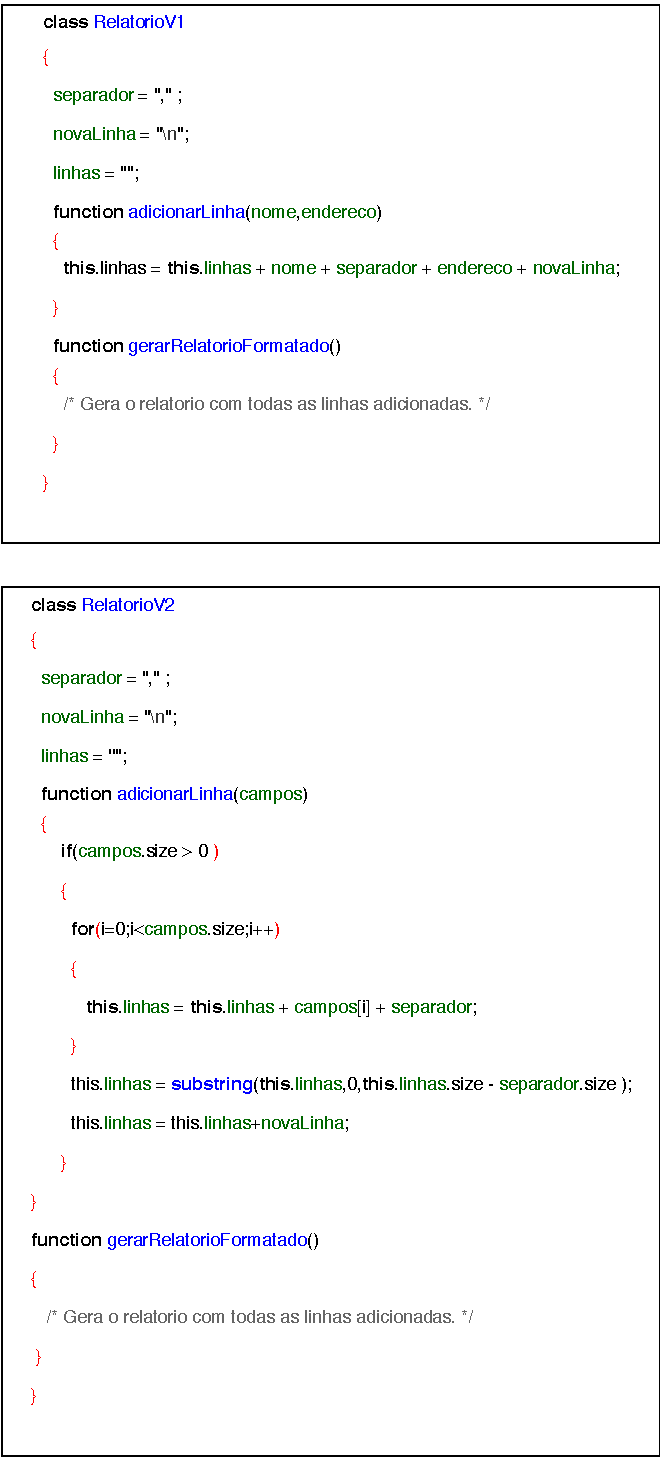
\includegraphics{capitulo_divida/ExemploDividaCodigo.pdf} 
  \caption{Exemplo de dívida técnica em código fonte. }
  \label{fig:cap1_exemplo_divida_codigo} 
\end{figure}


 
 Nosso segundo exemplo de dívida técnica está relacionado com o banco de dados de uma aplicação. De acordo com \cite{elmasri2016fundamentals} as restrições de integridade são mecanismos que os sistemas gerenciadores de banco de dados fornecem  para que os usuários possam definir regras a respeito dos dados armazenados de forma que eles se mantenham consistentes e representem corretamente a realidade modelada. Um tipo de restrição muito comum são as de integridade referencial. Nesse tipo de restrição, basicamente, o banco de dados garante que para cada linha em uma relação onde exista uma chave estrangeira, sempre exista a linha correspondente na relação associada. O princial papel desse tipo de restrição de integridade é evitar situações no qual uma chave estrangeira faça referência a um dado que não existe na tabela associada. Na Figura ~\ref{fig:cap1_exemplo_integridade_referencial} há um exemplo de um modelo em que as restrições de integridade seriam úteis para garantir a consistência dos dados. Esse modelo contém três tabelas: Aluno, Curso e Histórico. Na tabela Histórico temos duas chaves estrangeiras chamadas de $ALUNO\_ID$ e $CURSO\_ID$. Caso alguns alunos ou cursos, que estejam presentes na tabela Histórico, sejam removidos, as linhas que contém referências a esses elementos não mais farão sentido dentro do modelo e indicarão a existência de dados inconsistentes. Uma forma de evitar esse problema é criar uma restrição de integridade de tal forma que, antes de remover alguma linha nas tabelas Aluno e Curso, o próprio sistema gerenciador do banco de dados verifique se isso não gerará linhas órfãs na tabela Histórico. Nesse exemplo é simples identificar qual restrição de integridade é necessária para garantir a consistência do modelo. Entretanto, em situações reais, a quantidade de tabelas e restrições necessárias podem ser muito grandes. Em algumas situações nem todas as restrições são devidamente mapeadas e implementadas no banco de dados devido à alguma restrição de recurso. Quando isso acontece, há a aquisição de uma dívida técnica. A dificuldade adicional gerada por essa dívida ocorre quando é necessário incluir alguma restrição que não foi anteriormente aplicada. Isso pode levar a necessidade de adaptar e testar um número grande de partes do sistema que de alguma forma utilizam as tabelas relacionadas com a restrição. É possível inclusive que seja necessário realizar alterações nessas partes para que elas se adequem a inclusão das novas restrições de integridade. Isso pode levar a um custo substancial gerado pela necessidade de um conjunto de alterações em cascata. 
 
 \begin{figure}[!h]
  \centering
  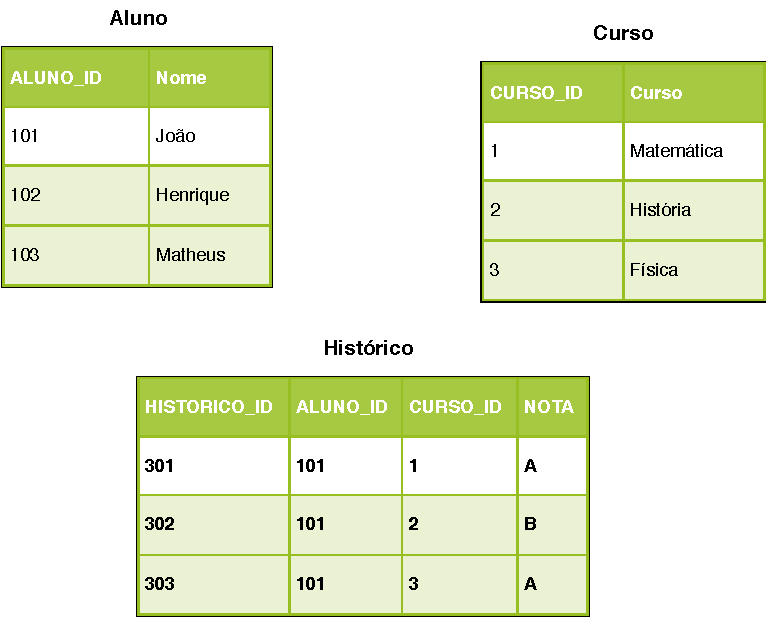
\includegraphics{capitulo_divida/ExemploIntegridadeRelacional.pdf} 
  \caption{Exemplo de dívida técnica em banco de dados. }
  \label{fig:cap1_exemplo_integridade_referencial} 
\end{figure}
 
 



Utilizaremos um exemplo relacionado às atividades de testes durante o processo de desenvolvimento de software para concluir nossa ilustração a respeito das dívidas técnicas. Existem diversos tipos de testes que podem ser realizados em um software. Dentre esses tipos, os testes unitários são aqueles que têm como objetivo validar se as menores unidades estão funcionando individualmente como o esperado\cite{cheon2002simple,runeson2006survey}. Esses testes consistem, basicamente, em acionar essas unidades fornecendo uma entrada e verificar se a saída corresponde ao que foi especificado.  Essas unidades podem ser métodos, classes, funcionalidades ou módulos. Em um cenário perfeito, todas as unidades do software deveriam ser testadas para todas as entradas possíveis. Naturalmente, devido à quantidade de recursos necessários, isso não é possível em todos os casos. Sendo assim, existe a necessidade de selecionar quais testes serão criados. Essa seleção pode ser feita de diversas formas. Seja pela priorização das unidades mais importantes ou pela escolha das entradas que são mais prováveis de serem fornecidas durante o funcionando do sistema. Além disso, é necessário que haja uma compatibilização entre a quantidade de testes que serão criados e a quantidade de recursos disponíveis. Haverá a aquisição de uma dívida técnica caso o número de testes criados não seja compatível com o nível de qualidade necessário para o software e no futuro seja necessário criar mais testes. A dificuldade adicional gerada pela existência dessa dívida técnica é causada pelo fato de que possivelmente seja necessário realizar refatorações\cite{mcintosh2014impact,morales2016finding} nas unidades do sistema para facilitar ou até mesmo tornar possível a criação desses testes. Isso ocorre porque a estrutura dessas unidades pode ter sido construída de forma que seja impossível testar determinados comportamentos. Na Figura \ref{fig:cap1_exemplo_refatoracao_teste_unitario} exibimos duas versões de uma mesma classe. Na primeira versão, existe uma dificuldade em testar o método calculaImposto. Isso acontece, pois, essa versão do método tem duas responsabilidades: calcular o imposto e inserir o resultado no banco de dados. Caso um teste unitário fosse escrito para essa versão, seria necessário fornecer uma conexão de banco de dados válida. Além disso, a inserção de dados em um banco de dados iria de encontro com os objetivos dos testes unitários já que o teste abrangeria um escopo maior do que uma unidade. Esses problemas não são encontrados na versão 2 do método calculaImposto. Nessa versão, a conexão com o banco de dados é um parâmetro do método. Assim, é possível criar um teste onde fosse utilizada uma conexão fictícia de banco de dados ou um Mock\cite{mackinnon2000endo,kaczanowski2012practical,acharya2014mastering}. Esse teste verificaria se o método calculaImposto está tendo um comportamento conforme a especificação do software. A refatoração que levou o método da versão 1 para a versão 2 também exigirá que todas as referências ao método calculaImposto sejam alteradas. Logo, haverá uma dificuldade adicional para realizar essa alteração se compararmos a dificuldade de realizá-la no momento em que a versão 1 foi criada. 
 
 
  \begin{figure}[H]
  \centering
  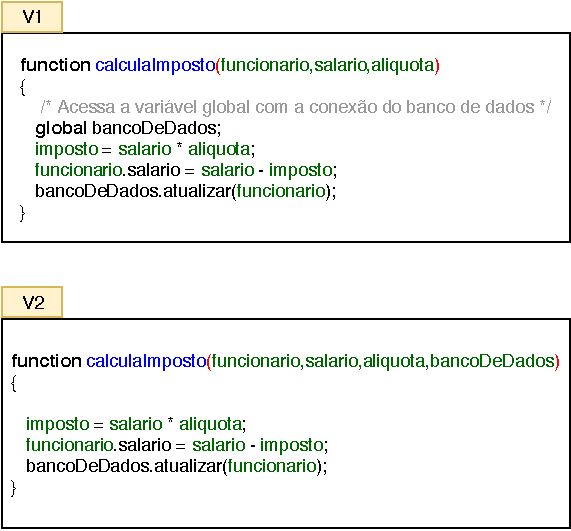
\includegraphics{capitulo_divida/ExemploRefatoracaoParaTesteUnitario.pdf} 
  \caption{Exemplo de refatoração para viabilizar a criação de um teste unitário. }.
  \label{fig:cap1_exemplo_refatoracao_teste_unitario} 
\end{figure}








\section{Definição da dívida técnica}
\label{definicao_divida_tecnica}

Em 1992 Cunningham\cite{cunningham1993wycash} criou o termo dívida técnica da seguinte forma:
 

\say{\textit{Although immature code may work fine and be completely acceptable to the customer, excess quantities will make a program unmasterable, leading to extreme specialization of programmers and finally an inflexible product. Shipping first time code is like going into debt. A little debt speeds development so long as it is paid back promptly with a rewrite. Objects make the cost of this transaction tolerable. The danger occurs when the debt is not repaid. Every minute spent on not-quite-right code counts as interest on that debt. Entire engineering organizations can be brought to a stand-still under the debt load of an unconsolidated implementation, object- oriented or otherwise.}}


Apesar de Cunningham ser considerado o criador da metáfora, outros autores escreveram previamente a respeito das dificuldades de manutenção e evolução causadas por problemas de design. Um exemplo é o conjunto de leis da evolução de software criadas por Lehman \cite{lehman1980programs,lehman1996laws} em 1980. Nesse trabalho, o autor analisa estudos prévios sobre processos de programação e acompanha a evolução  do  sistema operacional OS/300 durante um período de 20 anos. Com os dados obtidos, são formuladas 8 leis que descrevem algumas características observadas durante a evolução de um software. Algumas dessas leis apresentam conceitos claramente muito semelhantes aos utilizados para descrever a metáfora da dívida técnica. Especialmente, as leis II e VII, transcritas a seguir.

\subsubsection{II - \textit{Increasing Complexity}}
\textit{``As a program is evolved its complexity increases unless work is done to maintain or reduce it."}

\subsubsection{VII - \textit{Declining Quality}}
\textit{``E-type programs will be perceived as of declining quality unless rigorously maintained and
adapted to a changing operational environment."}

A lei II descreve de forma indireta a dívida técnica de design e arquitetura. Esses tipos de dívida técnica foram descritos nas seções \ref{tipo_td_design} e \ref{tipo_td_arquitetura} respectivamente. Enquanto isso, a lei VII está relacionada às dívidas técnicas de tecnologia, descritas na seção \ref{tipo_td_tecnologia}. Um sistema chamado de \textit{E-type} é aquele efetivamente utilizado em um contexto real, ou seja, as leis descritas por Lehman não se aplicam a sistemas que não operam em um contexto sujeito a mudanças.  Apesar de haver contestações a respeito do uso do termo ``leis", este trabalho permitiu observar como a percepção dos usuários e programadores muda à medida que o tempo passa e o software evolui.  

Apesar da existência de relatos semelhantes na década de 80 e da criação da metáfora em 1992, apenas a partir do ano de 2006 \cite{mar2006technical} que a analogia volta a ser discutida e estudada cientificamente. Inicialmente houve um esforço por parte dos pesquisadores em criar uma definição precisa do que é uma dívida técnica. Essa definição inicial indicava que uma dívida técnica deveria ser algo invisível para o usuário final do software. A Figura \ref{fig:cap1_panorama_td} apresenta uma adaptação da representação gráfica dessa definição. 

Além da expansão do conceito para incluir diversos tipos de dívida conforme veremos na sessão \ref{sec:tipos_td}, houve, com o objetivo de torná-la menos ambígua, também um aprimoramento da definição em si. Essa evolução permitiu diferenciá-la do simples déficit de qualidade de um software, tornar o conceito mais claro, e principalmente, facilitar a identificação do que não se trata de uma dívida técnica. Na Figura \ref{fig:cap1_panorama_td} há um resumo a respeito desse estágio de evolução do conceito. Nele, houve uma tentativa de separar as dívidas técnicas de outros aspectos de qualidade do software. O resultado foi que apenas os problemas de qualidade que são invisíveis para o usuário final foram definidos como dívida técnica. Objetivo dessa separação é evitar a diluição do conceito. Essa diluição faria com que uma quantidade demasiadamente grande de situações fossem consideradas dívidas técnicas. Isso dificultaria a criação de pesquisas mais aplicadas a respeito de técnicas e ferramentas para o gerenciamento da dívida técnica. Com isso, ficou definido que as dívidas técnicas são problemas de qualidade interna do software. A qualidade interna engloba os aspectos que não são visíveis para o usuário final do software\cite{al2010quality}. Na Figura \ref{fig:cap1_hierarquia_qualidade} há uma indicação do lugar das dívidas técnicas dentro do contexto de qualidade de software.


 \begin{figure}[H]
  \centering
  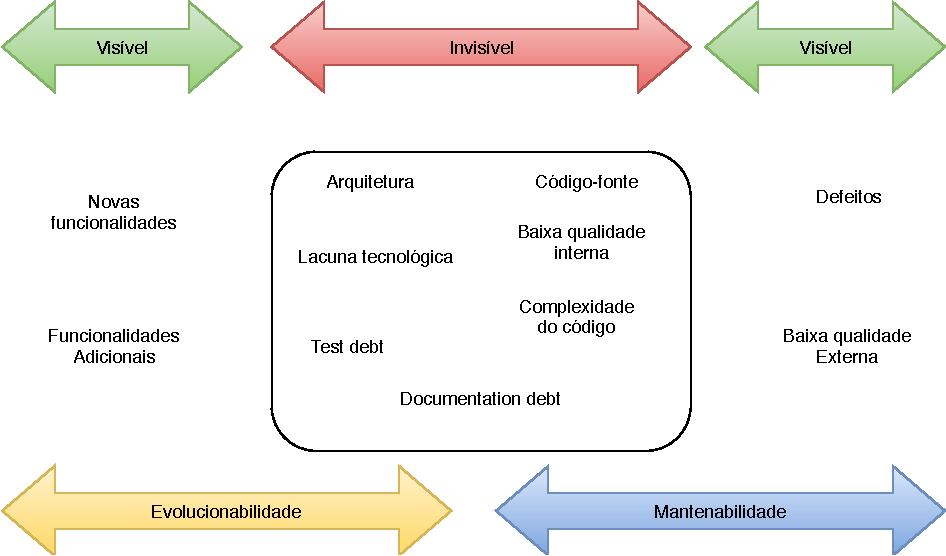
\includegraphics{capitulo_divida/DefinicaoTD.pdf} 
  \caption{Panorama da dívida técnica. Adaptado de \cite{kruchten2013technical}. }.
  \label{fig:cap1_panorama_td} 
\end{figure}

 \begin{figure}[H]
  \centering
  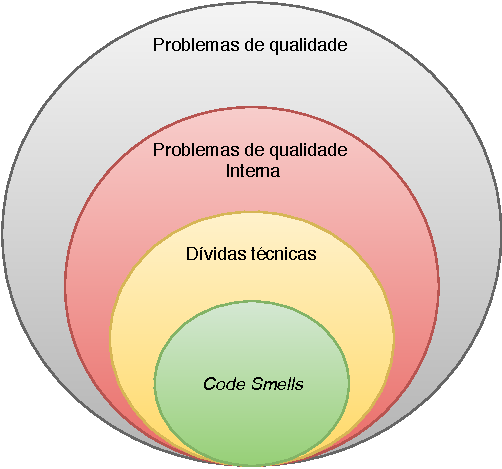
\includegraphics{capitulo_divida/HierarquiaProblemas.pdf} 
  \caption{Localização da dívida técnica na hierarquia dos problemas de qualidade de software. }.
  \label{fig:cap1_hierarquia_qualidade} 
\end{figure}


Com o aumento da popularidade dessa metáfora, novos tipos de dívida técnica surgiram. Alguns desses novo tipos não se enquadravam nessa definição, como, por exemplo, as dívidas de usabilidade e os defeitos. Isso fez com que os pesquisadores tivessem que abandonar a procura por uma definição precisa. Ao invés disso, foi adotada uma definição mais flexível e que permitisse que essa metáfora pudesse ser utilizada em diferentes situações. Um dos resultados desse esforço em busca de uma expansão do conceito foi a seguinte definição criada por Kruchten et al.\cite{kruchten2013technical}:

\say{A unifying perspective is emerging of technical debt as the invisible results of past decisions about software that affect its future. The affect can be negative in the form of poorly managed risks but if properly managed can be seen in a positive light to add value in the form of deferred investment opportunities.  }

Fica evidente, nessa definição, a preocupação em não mais restringir as dívidas técnicas à problemas  presentes no código fonte do software. Um dos motivos disso é a necessidade de diferenciá-las do conceito de \textit{Bad Smells} criado por Fowler\cite{fowler2009refactoring} e que se tornou muito popular na comunidade de desenvolvimento de software\cite{olbrich2009evolution}. Um ``\textit{smell}'' é uma violação à algum princípio do desenho de software orientado a objetos. Alguns exemplos de \textit{smells} são código duplicado, classes muito extensas ou muito curtas e métodos demasiadamente longos\cite{van2002java}. Essencialmente, um \textit{Bad Smell} é uma dívida técnica no código orientado a objetos\cite{poliakov2015systematic}. Como evidenciado na Figura \ref{fig:cap1_hierarquia_qualidade} todos os \textit{Bad Smells} são dívidas técnicas, mas nem toda dívida técnica é um \textit{Bad Smell}.


Tendo sido superada essa fase de definição do termo, a comunidade agora procura por teorias e técnicas comprovadamente eficazes para o gerenciamento e identificação da dívida técnica \cite{falessi2014technical}.





\subsubsection{Sinônimos}

A dívida técnica, por ser um fenômeno aparentemente onipresente nos projetos de software\cite{lim2012balancing,brown2010managing}, foi percebida e chamada de diversas formas pelos profissionais e pesquisadores. Existem ao menos duas razões para que esses sinônimos sejam devidamente documentados. A primeira delas está relacionada com a pesquisa bibliográfica a respeito do tema. Existem diversos trabalhos com resultados relevantes e que não usam diretamente o termo dívida técnica\cite{fowler2018refactoring,lanning1994modeling,lindgren2012bridging,smit2011code}. A segunda razão é a de permitir que seja traçado um retrospecto a respeito do assunto incluindo informações anteriores à definição do termo em 1992 por Cunningham\cite{cunningham1993wycash}. Poliakov realizou uma revisão sistemática a respeito dos sinônimos da dívida técnica\cite{poliakov2015systematic}. Um dos resultados dessa revisão sistemática é um catálogo com os sinônimos para a dívida técnica encontrados na literatura. Na tabela \ref{tab:tabela_sinonimos}, apresentados um resumo desse catálogo.

\begin{table}[H]
\centering
\begin{tabular}{|l|}
\hline
\multicolumn{1}{|c|}{Sinônimos}                  \\ \hline
Shortcut                                   \\ \hline
Code Smells / Design principles violation                                \\ \hline
Workaround / Hack                          \\ \hline
Grime                                        \\ \hline
Software aging                                     \\ \hline
Spaghetti code                                        \\ \hline
\end{tabular}
\caption{Sinônimos do termo dívida técnica. Adaptado de \cite{poliakov2015systematic}}
\label{tab:tabela_sinonimos}
\end{table}

\section{A metáfora}

A metáfora dívida técnica surgiu inicialmente como uma forma de explicar a necessidade de evitar que código de má qualidade se espalhe pelo software a ponto de tornar sua evolução inviável\cite{cunningham1993wycash}. Uma das vantagens da utilização dessa metáfora é a sua capacidade de facilitar a justificativa para a disponibilização de recursos para a realização de atividades que não estejam diretamente ligadas à adição de novas funcionalidades ou correção de defeitos.  A utilização de uma analogia com aspectos financeiros pode ser eficaz para explicar para pessoas sem conhecimento em desenvolvimento de sistemas a necessidade de empregar recursos para evitar o acúmulo de juros. Ainda assim,  apesar de ser apropriada, a metáfora dívida técnica tem diversas diferenças em relação a sua contrapartida no contexto financeiro e essas diferenças precisam ser consideradas durante seu gerenciamento. Uma delas é a impossibilidade de calcular previamente os juros a serem pagos. É difícil calcular com exatidão qual o esforço extra necessário para evoluir e manter o software devido a existência de uma dívida técnica. Apesar de algumas contribuições relevante\cite{singh2014framework,seaman2011measuring,curtis2012estimating}, até mesmo a criação de estimativas é um desafio devido à imprevisibilidade a respeito do contexto no qual o software será desenvolvido no futuro. Isso acontece principalmente porque, quase sempre, não é possível determinar se uma parte do código-fonte será ou não alterada. A quantidade de juros será proporcional à frequência de alterações relacionadas na parte do código com dívida técnica. Além disso, mesmo que existam dívidas técnicas nessa parte, não haverá incidência de juros caso não haja nenhuma alteração no futuro. Devido a essa incapacidade de prever se uma dívida técnica gerará ou não juros, alguns autores como Schmid, K\cite{schmid2013limits} diferenciam as dívidas técnicas como efetivas ou potenciais. Uma dívida potencial é aquela que está associada a uma expectativa de  existência de juros. Ou seja, ela ainda não trouxe nenhum esforço adicional para o desenvolvimento do software. Enquanto isso, uma dívida técnica efetiva é aquela que já está gerando dificuldades adicionais nas tarefas de desenvolvimento e manutenção do software. Apesar das diferenças, a metáfora da dívida técnica é uma forma eficaz de evidenciar a necessidade de manter um equilíbrio entre a existência de recursos limitados e a preocupação de manter viável a evolução do software a médio e longo prazo.



\subsection{Elementos da metáfora}
\label{elementos_td}

Assim como na área financeira, os principais conceitos relacionados a dívida técnica são o principal e os juros. Entretanto, além desses conceitos, existem outros. De acordo com \cite{li2015systematic} existe uma lista de conceitos utilizados para descrever a dívida técnica e suas consequências. A seguir iremos descrever alguns desses conceitos.


\subsubsection{Principal}
O principal corresponde ao resultado gerado pelas atividades feitas de forma não ideal e que, consequentemente, não apresentam um nível de qualidade compatível com o projeto. No caso da dívida técnica no código, o principal será o trecho ou trechos do código que não estão de acordo com as boas práticas de desenvolvimento ou que não estão de acordo com critérios de qualidade adotados pela equipe de desenvolvimento. O valor do principal é equivalente ao esforço necessário para corrigir algum aspecto do software que não esteja adequado. Usando novamente o exemplo da dívida técnica no código, o valor do principal é equivalente ao esforço necessário para alterar o código, de forma que ele fique de acordo com os padrões de qualidade necessários para o projeto.

Uma característica importante a respeito do valor do principal é que ele se altera com o passar do tempo. Isso acontece por diversas razões. Uma delas é a adição de novos artefatos ao software a medida que ele evolui. Com isso, nos casos em que esses artefatos também terão de ser alterados devido ao pagamento do principal, o esforço total necessário será maior. Outra razão para a variação temporal do esforço necessário para eliminar o principal é a possibilidade de que, devido ao tempo passado, a equipe já não esteja tão habituada com a parte do software onde a mudança precisa ser feita. As regras de negócios associadas com o código a ser alterado podem ter sido discutidas em um período de tempo muito anterior ao momento onde o pagamento do principal será feito. Além disso, é possível que até mesmo a tecnologia utilizada possa já não ser dominada pela equipe como era no momento em que o principal foi inserido no código. 

Há uma semelhança entre a variação temporal do valor do principal e o conceito financeiro de correção monetária de uma dívida. De acordo com Schmidt\cite{santos2007teoria}, a correção monetária é um método de tornar real o valor monetário das contas permanentes das demonstrações contábeis. Essa correção é realizada por meio de algum índice como a inflação acumulada em um determinado período de tempo. Em ambos os casos, há uma tendência de aumento da dívida com o passar do tempo. Caso esse aumento não seja gerenciado, pode chegar a um cenário onde seu pagamento se torne inviável. 

\subsubsection{Juros} 

No contexto financeiro, os juros são os valores a serem pagos a um credor após a aquisição de um empréstimo. Dessa forma, podem ser definidos como o preço a ser pago para permanecer com uma determinada quantia. Enquanto essa quantia não for paga para o credor, os juros serão pagos na forma de uma porcentagem relativa ao valor ainda devido. Essa porcentagem não é igual para todos os credores. Assim como qualquer outro produto, o preço do empréstimo varia, ou seja, existem empréstimos com um preço maior ou menor que outros. Assim como existem dívidas técnicas que produzem mais ou menos juros.

No contexto da dívida técnica, os juros são todo o esforço adicional nas atividades de desenvolvimento software causado pela existência da dívida técnica. Por exemplo, no caso da dívida técnica de arquitetura, os juros serão toda a dificuldade causada por uma característica da arquitetura do software que não esteja de acordo com os padrões de qualidade definidos para o software. Essa dificuldade pode estar relacionada com o tempo necessário para se adicionar um novo elemento na arquitetura por exemplo. Enquanto o principal não for pago, isto é, enquanto o problema arquitetural não for resolvido, a equipe terá de lidar com as dificuldades causadas pelos juros. A Figura \ref{fig:juros} ilustra essa definição dos juros da dívida técnica. 

\begin{figure}[H]
  \centering
  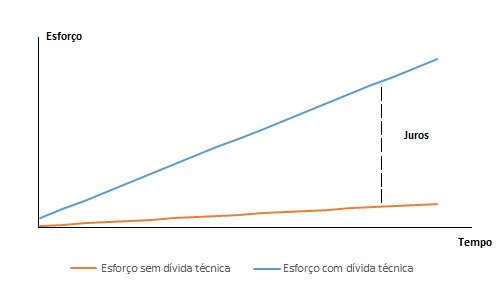
\includegraphics[width=13.28cm,height=7.65cm]{juros.png} 
  \caption{Representação dos juros como o esforço adicional causado pela dívida técnica. }.
  \label{fig:juros} 
\end{figure}



\subsubsection{Probabilidade dos juros}

Muitas vezes existe uma incerteza em relação aos juros causados pela existência da dívida técnica. Essa incerteza está na ocorrência ou não desses juros como também em seu valor.  
Isso acontece, pois o esforço futuro necessário para desenvolver o software depende de fatores que não são conhecidos \textit{a priori}. Até mesmo não é possível afirmar que uma determinada parte do software, relacionada a uma dívida técnica, terá de ser alterada no futuro. 

\subsubsection{Ponto de quebra}

É chamado ponto de quebra o instante no tempo onde os juros da dívida técnica se acumulam de tal forma que tornam inviável a realização das atividades de evolução do software \cite{chatzigeorgiou2015estimating}. Em alguns casos, ao atingir esse ponto, a equipe de desenvolvimento cogita a hipótese de abandonar o projeto atual e recomeçar um novo do início. Esse processo é algumas vezes chamado de \textit{like-to-like migration}.  Apesar de parecer uma alternativa plausível, essa opção apresenta uma série de pontos fracos. Alguns deles são o custo elevado de reconstrução do software, a necessidade de considerar atualizações no conjunto de requisitos originais e a necessidade de utilizar tecnologias mais atuais e que consequentemente exigem treinamento e adaptação\cite{sterling2010managing}. Ou seja, o esforço necessário para a criação de uma solução do tipo \textit{like-to-like} normalmente é subestimada e irá custar mais do que o imaginado. 
 

\section{Classificações da dívida técnica}
\label{classificacoes_divida_tecnica}

Uma forma recorrentemente encontrada na literatura de classificar a dívida técnica é como intencional e não intencional\cite{sterling2010managing,brown2010managing,klinger2011enterprise}. A dívida técnica não intencional é aquela que as pessoas relacionadas ao desenvolvimento e evolução do software não sabem que a estão gerando. Esse desconhecimento pode ser devido à falta de experiência, conhecimento ou cuidado. Por outro lado, a dívida técnica intencional é aquela devidamente documentada e usada como uma ferramenta para alcançar um objetivo de curto prazo e que não seria possível caso a atividade fosse realizada de forma a atender o padrão de qualidade estabelecido.  Além disso, existe um planejamento indicando como e quando essa dívida técnica será paga. Enquanto que a dívida técnica não intencional sempre é negativa e expõe deficiências nas atividades de desenvolvimento do software, a dívida técnica intencional pode ser uma aliada estratégica para aumentar a produtividade de uma equipe. O gerenciamento da dívida técnica não tem como objetivo eliminar completamente a existência da dívida técnica nos projetos de software. Ao invés disso, ela pode ser resumida como a busca pelo equilíbrio entre a aquisição e o pagamento da dívida de forma que ela se mantenha controlada e benéfica para o projeto. 

Dentre as dívidas técnicas intencionais, podemos definir uma subcategoria chamada \textit{self-admitted technical debt}. Essa é uma forma de dívida técnica onde o programador indica explicitamente nos comentários do programa que seu código contém dívida técnica. Essas dívidas são descritas no próprio código da aplicação por meio de comentários. É chamada de \textit{self-admitted} porque o próprio programador admite que a solução apresentada não é adequada. Um dos trabalhos que abordam essa forma de dívida técnica\cite{maldonado2015detecting} disponibilizou um banco de dados com  33k+ comentários com \textit{self-admitted technical debt} em projetos de código livre.


As dívidas técnicas \textit{self-admitted} ganharam certa atenção na literatura. Um exemplo disso é o trabalho de Maldonado et al.  \cite{maldonado2015detecting}. Nesse estudo os autores  investigaram quais são os tipos de SATD e quantificam a ocorrências desses tipos em projetos de software livre. Identificar os tipos de SATD  é importante pois, 1) ajuda a comunidade a entender as limitações a respeito da compreensão sobre SATD, 2) complementa as técnicas existentes de detecção de dívida técnica, 3) fornece uma melhor compreensão a respeito do ponto de vista dos desenvolvedores sobre a dívida técnica. Para a realização deste estudo foram analisados 5 projetos de código fonte aberto de diferentes domínios de aplicação. A extração dos comentários do código dessas aplicações foi realizada em duas etapas. Na primeira, foram excluídos automaticamente, por meio de um programa, os comentários que tinham baixa chance de conter informações a respeito da dívida técnica. Como resultado, foram selecionados 33.093  comentários. Em seguida, os comentários restantes foram analisados manualmente por um experiente desenvolvedor de software.  Após a análise manual, foram selecionados 2.457 comentários que estavam realmente relacionados com a dívida técnica nos 5 projetos analisados. Esses comentários estão foram inseridos em um banco de dados disponibilizado publicamente pelos autores. Como resultado, foram identificadas 5 categorias de SATD: Design, defeitos, documentação, requisitos e testes. Os tipos design e requisitos são os mais presentes nos projetos analisados. Os SATD de design representam de 42\% a 84\% dos comentários enquanto que os SATD de requisitos representam de 5\% a 45\% dos comentários. Os autores indicam a utilização de técnicas de processamento de linguagem natural como um possível caminho para avançar na pesquisa sobre SATD.

\section{Tipos de dívida técnicas}
\label{sec:tipos_td}

O termo dívida técnica foi inicialmente utilizado para descrever problemas relacionados ao código.  Entretanto, posteriormente, foi percebido que ele pode ser utilizado para descrever problemas relacionados com outros aspectos do desenvolvimento de software. A seguir, iremos descrever alguns dos tipos de dívida técnica mais citados na literatura.

\subsection{Código}

A dívida técnica de código está relacionada aos problemas  de organização e qualidade encontrados no código do software. Esses problemas são mais simples do que os apresentados na seção \ref{tipo_td_design}. Normalmente estão associados a não conformidade com o estilo de código definido ou reconhecidamente adequado pela comunidade que utiliza a linguagem de programação do projeto. Além disso, o impacto negativo causado pelas dívidas técnicas de código tem o escopo reduzido a classe, ao método ou ao bloco de código onde elas se encontram.  Podemos citar, como exemplo de dívida técnica relacionada ao código, a existência de duplicação, complexidade desnecessária e a não aderência aos padrões de estilos definidos para o software. A ferramenta Sonar Qube \cite{campbell2013sonarqube} possui um plugin capaz de detectar uma grande quantidade de tipos diferentes de dívida técnica de código. Essas dívidas são organizadas em categorias como testabilidade, reusabilidade e segurança. 


\subsection{Testes}


As dívidas técnicas de testes podem ocorrer em duas situações. A primeira delas é quando há uma quantidade insuficiente de testes. Isso faz com mudanças futuras no software possam se tornar mais difíceis devido a necessidade de realização de testes de regressão. A segunda situação que pode gerar dívida técnicas de testes é quando o código dos testes é escrito de forma inadequada. Segundo Wiklund et al.\cite{wiklund2012technical}, isso acontece porque as organizações geralmente negligenciam a qualidade do código, design e documentação quando produzem o software responsável pela automatização dos testes. Isso gera um acúmulo da dívida técnica causando problemas na utilização, extensão e manutenção destes sistemas.  Ainda segundo  Wiklund et al., existem quatro principais razões para a aquisição de dívidas técnicas no código dos testes automatizados. A primeira é a de que o reuso e o compartilhamento das ferramentas de automatização de testes são assuntos importantes e precisam ser considerados no gerenciamento da dívida técnica. A segunda observação está relacionada a infraestrutura do ambiente de automatização dos testes. Diferenças no ambiente de testes e no ambiente de produção podem causar resultados incorretos. A terceira observação se refere a excessiva generalidade das ferramentas de automação. A existência de muitas configurações induz o usuário a cometer erros na utilização dessas ferramentas. Por fim, as práticas de desenvolvimento de código para automatização de testes são menos rigorosas quando comparadas as utilizadas no código das outras partes do software. Esse fato naturalmente faz com que o acúmulo da dívida técnica nos sistemas de automação de testes seja maior. 

Szabados et al.\cite{szabados2015technical} apresenta estimativas do esforço necessário para corrigir as dívidas técnicas em uma amostra de projetos de automatização de testes na área de telecomunicações. Estes projetos são construídos com a linguagem TTCN que é amplamente utilizada para a criação de suítes de testes para protocolos de comunicação. Os projetos foram disponibilizados no endereço www.ttcn-3.org. Para estimar o esforço necessário para corrigir cada tipo de code smell foi utilizada o método Delphi ou o Planning Poker \cite{grenning2002planning}. Em ambos os métodos, os especialistas são consultados sucessivamente a respeito de uma estimativa. Em cada uma das consultas, os especialistas que fornecerem as menores ou maiores estimativas argumentam porque  as forneceram. Após isso, o grupo é consultado novamente. Esse processo é repetido até que as diferenças entre as estimativas fornecidas sejam pequenas o suficiente.  A dívida técnica presente em cada projeto foi identificada utilizando code smells. Utilizando o método Delphi foram definidas as estimativas em homens/hora para corrigir cada um dos tipos de code smell em um cenário fácil, médio e difícil. Ao final, foi calculado o esforço necessário para corrigir a dívida técnica em cada um dos projetos analisados. Foi identificado que em alguns casos, seriam necessárias mais do que 50 mil homens/hora para realizar a correção. Os autores concluem que existe uma quantidade substancial de dívida técnica nos projetos de automatização de testes analisados. Em alguns casos, apenas a correção da dívida técnica levaria anos para ser concluída. 



\subsection{Documentação}

 A dívida técnica de documentação é caracterizada pela  inexistência de documentação, documentação desatualizada ou documentação inadequada. Esse tipo de dívida técnica pode trazer impactos negativos para o projeto de software nos casos onde funcionalidades precisem ser adicionadas ou alteradas. O tempo necessário para realizar essas atividades pode ser sensivelmente maior em comparação com o cenário onde haja documentação adequada. Isso ocorre, pois, os responsáveis por realizar essas atividades precisarão reservar tempo para procurar em fontes não estruturadas as informações necessárias para concluí-las. Além disso, existe o risco que sejam assumidas soluções baseadas em documentação incorreta ou atualizada. Isso pode gerar atrasos e aumentar a quantidade de recursos utilizados.

\subsection{Defeitos}

Assim como existem na literatura divergências a respeito do que deve ser considerado como dívida técnica, existem divergências a respeito do que não deve ser considerado como dívida técnica. Alguns estudos explicitamente definem que defeitos devem ser considerados como dívida técnica \cite{davis2013driving,guo2011portfolio,xuan2012debt}. Esses autores restringem esses defeitos a aqueles que não apresentam grandes dificuldades para o usuário ou possuem algum caminho alternativo para contorná-los. Já alguns autores argumentam que devem ser considerados como dívida técnicas apenas elementos que não estejam visíveis para o usuário final\cite{kruchten2013technical}. 

\subsubsection{Arquitetura}
\label{tipo_td_arquitetura}

A dívida técnica arquitetural é uma violação no código do software em relação a alguma característica arquitetural pré-definida tal tais como modularidade, portabilidade e escalabilidade. Além disso, são consideradas dívidas técnicas de arquitetura as violações de restrições impostas pelos desenvolvedores de software tais como o isolamento entre módulos específicos e  a proibição de acesso direto ao banco de dados.  Um exemplo de dívida técnica arquitetural é a presença de dependências proibidas entre  dois componentes. Neste trabalho \cite{martini2014architecture}, os autores apresentam uma taxonomia para as causas do acúmulo da dívida técnica arquitetural e um modelo para o processo de acúmulo e pagamento. Para criar essa taxonomia e esse modelo foi realizado um estudo de caso envolvendo cinco empresas de desenvolvimento de software.  O estudo de caso foi realizado em duas fases. A primeira fase consistiu em um estudo preliminar envolvendo apenas três das cinco empresas. Nesse estudo, foram realizados workshops com diferentes membros dessas empresas para identificar os principais desafios no gerenciamento da dívida técnica arquitetural. A segunda fase envolveu, além de representantes das cinco empresas, a análise de documentos e a realização de entrevistas mais informais. Ao final, os resultados foram apresentados e discutidos com 15 representantes das cinco empresas. Os fatores que levam ao acúmulo da dívida técnica arquitetural foram divididos em oito categorias: negócios, falta de documentação, utilização de código open source ou legado, desenvolvimento em paralelo, incerteza a respeito dos efeitos da refatoração, refatorações incompletas, evolução da tecnologia e fatores humanos. O estudo de caso mostrou que os modelos de acúmulo e pagamento da dívida técnica devem considerar que haverá um ponto no tempo onde o acúmulo excessivo da dívida gerará uma crise  no desenvolvimento do software de tal forma que o pagamento da dívida não poderá ser mais postergado. Ao atingir esse ponto crítico, é necessário que a dívida técnica seja paga. As equipes podem realizar pagamentos parciais ou totais antes de atingir esse ponto crítico para que ele seja adiado ou totalmente evitado. 


\subsection{Design}
\label{tipo_td_design}

Durante a história da programação orientada a objetivos, foram sendo observadas a existência de certas propriedades para que um código orientado a objetos possa ser entendido e alterado mais facilmente.  Dentre essas diversas propriedades, podemos destacar a necessidade de baixo acoplamento entre os elementos do software e a necessidade de alta coesão. Uma dívida técnica de design é caracterizada pela ocorrência de código que viola esses princípios de padrões reconhecidos como corretos para o desenvolvimento de software orientado a objetos.  



\subsection{Construção}
Algumas atividades comuns à tarefa de construção do software, tais como compilação de arquivos fonte e a análise e importação de dependências, atualmente são realizadas automaticamente por ferramentas de construção como Apache Ant\cite{de2015learning}, Maven\cite{goldman2007maven} e Gradle\cite{muschko2014gradle}. Essas ferramentas são capazes de obter da internet pacotes no qual o software seja dependente, executar e analisar os resultados de testes unitários, além de poderem ser configuradas para emitir relatórios com detalhes sobre o processo de construção.  Entretanto, é necessário que o software seja estruturado de forma a utilizar adequadamente as funcionalidades dessas ferramentas de automatização de construção. A dívida técnica de construção é caracterizada pela existência de características no software que não permitam a utilização das facilidades oferecidas por essas ferramentas. Logo, muitas das atividades de construção deverão ser realizadas manualmente, aumentando o esforço necessário para completá-las.  A busca por soluções para este tipo de dívida técnica tem se tornado popular no âmbito profissional devido à inerente busca por automatização dos processos de desenvolvimento de software\cite{morgenthaler2012searching}.

\subsection{Tecnologia}
\label{tipo_td_tecnologia}

Uma outra forma de dívida técnica está relacionada a evolução da tecnologia utilizada nos projetos.  Com o passar do tempo, novas ferramentas e tecnologias são criadas para tornar o desenvolvimento de software mais eficaz e eficiente. Logo, as tecnologias utilizadas se tornarão obsoletas com o passar do tempo. Quando essas tecnologias não são atualizadas ou substituídas, o esforço necessário para o desenvolvimento é maior em relação ao cenário onde as tecnologias mais recentes são utilizadas. Isso é o que caracteriza a existência de uma dívida técnica.

Para cada tipo de dívida técnica haverá uma estratégia diferente para o pagamento do principal. Para eliminar a dívida técnica de design é necessário realizar refatorações. Enquanto isso, para quitar a dívida técnica de documentação é necessário que a documentação atual seja atualizada, expandida ou reestruturada. 





\section{Gerenciamento da dívida técnica}

O gerenciamento da dívida técnica se assemelha ao gerenciamento de projetos. Existe uma série de atividades que precisam ser desempenhadas como identificação, análise, priorização e monitoramento. Apesar dessas atividades serem comuns ao gerenciamento da dívida técnica, existem diversas formas de desempenhá-las. Assim como no gerenciamento de projetos existem diversas técnicas diferentes que podem ser usadas em diversas atividades.

Caso o principal da dívida técnica não seja pago, os juros podem crescer a ponto de tornar a evolução do software insustentável. Logo, é importante que a dívida técnica seja devidamente gerenciada a fim de evitar que isso ocorra\cite{power2013understanding}. O gerenciamento da dívida técnica é um conjunto de atividades realizadas com o intuito de controlá-la de forma que ela não comprometa o desenvolvimento e evolução do software. De acordo com Zengyang Li. et. al.\cite{li2015systematic}, ele pode ser dividido em três atividades principais: a prevenção, identificação e o balanceamento entre aquisição e o pagamento da dívida.  A decisão de realizar uma atividade de forma a gerar uma dívida técnica normalmente é feita devido à limitação de recursos disponíveis para a realização da atividade.  Os responsáveis pelo gerenciamento do desenvolvimento e evolução do software precisam avaliar se o impacto causado pela aquisição da dívida será menor do que o benefício causado pela realização da atividade.  
 
As abordagens de gerenciamento da dívida técnica podem ser divididas em dois grupos. As abordagens que adaptam métodos financeiros e as abordagens específicas, especialmente criadas para o gerenciamento da dívida técnica. A seguir, descreveremos algumas das abordagens encontradas na literatura.


\subsection{Abordagens adaptadas da área financeira}

 A dívida técnica nada mais é do que uma metáfora que compara deficiências nos projetos de software com conceitos financeiros. Conforme descrito na seção \ref{elementos_td}, muitos dos conceitos utilizados para descrever a dívida técnica são originários da área financeira. Por causa disso, algumas das abordagens para o gerenciamento da dívida financeira foram adaptadas para serem utilizadas para gerenciar a dívida técnica. Um exemplo dessas abordagens é o gerenciamento de portfólio.  Em \cite{guo2011portfolio} Guo, et al., sugerem uma abordagem baseada em portfólios para gerenciar a dívida técnica. Um portfólio é o conjunto de investimentos que uma determinada empresa ou pessoa possui. Cada um desses investimentos possui um risco associado. Esse risco é uma medida para o quão provável é que o investimento não traga o retorno esperado. Quanto maior o risco, maiores as chances de o investimento não trazer o retorno esperado. O objetivo do gerenciamento de portfólio é escolher os itens desse conjunto de forma que o retorno seja o maior possível e o risco esteja dentro de um patamar pré-estabelecido. 


Apesar de a metáfora dívida técnica ter se mostrado útil como uma ferramenta de comunicação, existem muitas diferenças entre a dívida financeira e a dívida técnica que fazem com que a adaptação de abordagens de gerenciamento oriundas da área financeira seja de difícil realização. Em alguns casos, essa dificuldade é observada pelo fato de a área financeira utilizar métodos matemáticos complexos. Além disso, alguns conceitos financeiros, utilizados nessas abordagens, são de difícil mapeamento para o contexto de desenvolvimento de software. Um exemplo é o caso da técnica de precificação de opções definida por Black and Scholes \cite{chriss1996black}.  Essa técnica foi adaptada para ser utilizada em projetos de software \cite{benaroch1999case,alzaghoul2013cloudmtd,abad2015using}. Entretanto, mostrou-se de difícil utilização por pessoas sem um grande conhecimento na área financeira e em modelos matemáticos de análise. Mesmo tendo em vista a complexidade na utilização de algumas dessas abordagens, é possível que elas possam ser adaptadas com sucesso em projetos reais quando forem criadas ferramentas que automatizem seus cálculos e procedimentos. 


\subsection{Abordagens específicas}


Além das abordagens de gerenciamento originárias da área financeira, foram criadas abordagens  específicas para o gerenciamento da dívida técnica. Essas formas de gerenciamento foram criadas observando as necessidades específicas dos projetos de software em manter suas dívidas técnicas em níveis aceitáveis.



 Fernández-Sánchez, C et al.\cite{fernandez2015framework} sugerem uma proposta para o gerenciamento da dívida técnica. Nesta pesquisa, os autores iniciam a definição de um arcabouço para o gerenciamento da dívida técnica. Por meio de um mapeamento sistemático da literatura são definidos os elementos utilizados para o gerenciamento da dívida técnica e os como esses elementos são considerados pelos diferentes pontos de vista dos stakeholders. Os elementos mapeados pelos estudos foram:

\begin{itemize}
\item \textit{Identification of technical debt items}.
\item \textit{Principal Estimation}.
\item \textit{Interest estimation}.
\item \textit{Interest probability estimation}.
\item \textit{Technical debt impact estimation}.
\item \textit{Automated estimates}.
\item \textit{Expert Opinion}.
\item \textit{Scenario analysis}.
\item \textit{Time-to-market}.
\item \textit{When to implement decisions}.
\item \textit{Tracking technical debt over time}.
\item \textit{Visualizing technical debt}.
\end{itemize}

Os pontos de vista identificados foram engenharia, gerenciamento da engenharia e gerenciamento do negócio. A engenharia inclui processos de design e construção de software. O gerenciamento da engenharia envolve as atividades relacionadas ao planejamento e monitoramento. Por fim, as atividades de gerenciamento do negócio envolvem as estratégias, objetivos  e planejamento organizacional. O mapeamento sistemático também mostrou que todos os pontos de vistas estão majoritariamente focados nas técnicas de estimação da dívida técnica. Os autores acreditam que ao identificar quais conceitos estão relacionados ao gerenciamento da dívida técnica e como esses conceitos são utilizados, poderão, em trabalhos futuros, criar modelos concretos que auxiliem o gerenciamento da dívida técnica.

A abordagem mais madura de gerenciamento da dívida técnica encontrada na literatura é a definida por Seaman, C e Guo, T\cite{seaman2011measuring}. A Figura ~\ref{fig:seaman_framework}  ilustra a estrutura básica dessa abordagem. A TD list (\textit{Technical Debt List}) é um catálogo com as informações de todas as dívidas técnicas presentes no projeto. Esse catálogo inclui a data de identificação, descrição, localização, responsável, tipo, estimativa do principal, estimativa dos juros e estimativa da probabilidade dos juros ser efetivamente exercido. Todas as atividades de gerenciamento da dívida técnica atualizam ou obtêm informações desta lista. A abordagem criada pelos autores possui três atividades: Identificação, medição e monitoramento.  

As atividades de identificação e medição geram uma lista que contém, além das dívidas técnicas, informações sobre o principal e os juros. Na atividade de identificação, o software e os processos utilizados em sua construção são analisados a fim de encontrar dívidas técnicas. Cada ocorrência de dívida técnica é, então, inserida na TD List. Na identificação não é realizada uma análise mais profunda a respeito do principal e juros das dívidas. Ao invés disso, são utilizadas apenas estimativas superficiais como  simples, médio e difícil para designar o esforço necessário para correção. Na atividade de medição, é realizado um estudo mais completo a respeito do custo para pagamento das dívidas e dos juros relacionados. Esse estudo é realizado considerando as informações atuais a respeito do software e as futuras atividades de desenvolvimento e manutenção. Essa divisão entre identificação e medição é realizada pelo fato de a medição ser uma atividade cara. Logo, não faz sentido que ela seja realizada em dívidas que não serão pagas no curto prazo ou não tenham alto impacto no software. 

A atividade de monitoramento consiste em observar o ciclo de vida do software e incorporar ou remover da lista as dívidas a medida que elas forem sendo pagas ou novas dívidas forem sendo criadas.  Além disso, no monitoramento é feito um acompanhamento da evolução da dívida técnica do software a fim de manter o nível dentro de patamares aceitáveis.

 Além dessas atividades, os autores descrevem como deve ser o processo de decisão a respeito de quais dívidas devem ser pagas em uma release. Devem primeiro ser selecionadas as dívidas que estejam relacionadas ao componente ou componentes que serão alterados na release. Além disso, deve ser considerado o esforço, a probabilidade de que os juros tenham de ser pagos e os benefícios do pagamento da dívida. Esse framework não define explicitamente quais métodos ou ferramentas devem ser utilizados em cada atividade. Essa escolha é deixada para as pessoas que irão aplicá-lo. Apesar disso, os autores fornecem sugestões.


\begin{figure}[!h]
  \centering
  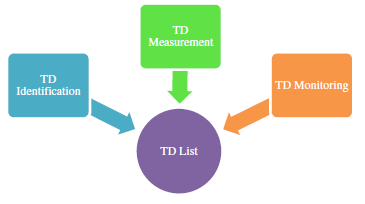
\includegraphics[width=9.66cm,height=5.4cm]{seaman_framework.png} 
  \caption{Framework para gerenciamento da dívida técnica. Adaptado de \cite{seaman2011measuring}.  }
  \label{fig:seaman_framework} 
\end{figure}


Para verificar a viabilidade de aplicação do framework, Seaman, C et. al., realiza um estudo onde são investigados os custos necessários para aplicar o arcabouço de gerenciamento
 \cite{guo2016exploring}. Nesse trabalho, os autores investigam o custo necessário para realizar o gerenciamento da dívida técnica em um projeto de software e como as informações sobre a dívida técnica influenciam o processo de decisão. Para realizar essa investigação é conduzido um estudo de caso em uma pequena empresa de desenvolvimento de software. O objetivo desse estudo de caso é identificar quais são os custos necessários para gerenciar a dívida técnica e como as informações sobre a dívida técnica contribuem para o processo de decisão.  O estudo de caso foi desenvolvimento em uma empresa que produz software empresarial, realiza consultoria e fornece serviços de treinamento. Uma equipe formada por nove profissionais foi monitorada durante o desenvolvimento de um software web de gerenciamento de embarcações. Foram realizadas as atividades de gerenciamento da dívida técnica propostas pelos autores. O foco nesse monitoramento estava no processo de decisão e como ele era influenciado pelas informações da dívida técnica. Por meio do estudo de caso, foram possíveis identificar quatro itens ou categorias de custo para o gerenciamento da dívida técnica. Essas categorias foram: a. identificação, b. análise e avaliação, c. comunicação e d. documentação. Sendo que a análise e avaliação foi a categoria com o custo mais alto. O custo do planejamento do projeto aumentou 70\% após a inclusão das atividades de gerenciamento da dívida técnica. Entretanto, este aumento significativo foi causado pelo custo de atividades iniciais que não serão repetidas em futuros projetos ou que terão o custo diminuído, como, por exemplo, as atividades de treinamento sobre a dívida técnica. O segundo objetivo do estudo foi identificar como as informações da dívida técnica influenciam o processo de decisão. O estudo de caso mostrou que as necessidades do cliente, a quantidade de recursos disponíveis, os juros da dívida técnica, o nível de qualidade do módulo e o impacto em outras funcionalidades são os fatores que influenciam o processo de decisão. Os autores concluem que o gerenciamento da dívida técnica na empresa do estudo de caso trouxe diversos benefícios. Isso foi evidenciado pelo fato de que o líder do projeto continuou utilizando a abordagem mesmo após o fim do estudo de caso. Além disso, o benefício causado pelo gerenciamento da dívida técnica se mostrou maior do que o custo de executá-lo. 

Neste trabalho\cite{oliveira2015managing} é realizada uma pesquisa-ação com o objetivo de avaliar em um cenário real a aplicação do framework de gerenciamento da dívida técnica proposto por Seaman, C e Guo, T\cite{seaman2011measuring}. A pesquisa-ação foi realizada em duas empresas brasileiras. A primeira desenvolve sistemas de gerenciamento de benefícios previdenciários. A segunda desenvolve sistemas de apoio para seguradoras. Ambas as empresas apresentaram indícios de existência de dívida técnica em seus projetos.  A pesquisa-ação é caracterizada pela interação entre pesquisadores e profissionais com o objetivo de resolver um problema real e ainda assim contribuir para uma área de pesquisa. A pesquisa-ação executada neste estudo foi realizada em cinco estágios: diagnose, planejamento, intervenção, avaliação e registro de aprendizado.  Foram realizados três seminários com cada uma das empresas. Nesses seminários foram apresentados os conceitos da dívida técnica e detalhes sobre framework que seria utilizado. 
Como fonte de dados para  a obtenção dos resultados desta pesquisa, foram utilizadas as anotações realizadas durante os seminários e questionários enviados aos participantes ao final de cada ciclo.  Foram observadas pelos pesquisadores e, confirmadas nos questionários, dificuldades por parte dos profissionais em mensurar as dívidas técnicas. Especialmente os juros, pois dependem da previsão de como a dívida afetará o projeto com o passar do tempo. Essa previsão é de difícil realização especialmente quando não há dados históricos.  Apesar disso, o estudo mostrou que os participantes acreditam que, ainda assim, essa avaliação, juntamente com a priorização da dívida técnica, precisa ser realizada por todo o time de desenvolvimento.  A maior parte das dívidas identificadas foram de design e código. Isso se justifica pelo fato de grande parte dos participantes do estudo serem arquitetos de software ou programadores. Os participantes também concordaram que o tempo necessário para a  inclusão de uma dívida técnica na \textit{technical debt list} foi razoável. Os autores concluem que as empresas irão continuar utilizando a estratégia de gerenciamento da dívida técnica utilizada mesmo após a finalização da pesquisa.  

\subsection{Dívida técnica como uma ferramenta estratégica}


Os estudos sobre gerenciamento da dívida técnica normalmente não consideram os aspectos estratégicos do projeto. Grande parte dos trabalhos encontrados na literatura consideram que a dívida já existe e precisa ser gerenciada. Existe uma ausência de trabalhos que abordem a possibilidade da dívida técnica ser utilizada como uma ferramenta  estratégica no gerenciamento de projetos de software. Como exemplo, muitas vezes uma dívida técnica é criada devido a uma necessidade  de disponibilizar rapidamente uma funcionalidade indispensável.  Pode ser feita uma relação entre essa situação e a utilização de técnicas de prototipagem evolutiva e desenvolvimento incremental que também permitem a disponibilização do software de forma incompleta ou não aderente aos padrões de qualidades exigidos para o produto final. Ainda assim,   são alternativas válidas para o projeto de desenvolvimento de software.  Logo, o gerenciamento da dívida técnica deveria ser feito de forma que haja um balanceamento entre essas possíveis  necessidades estratégicas e as necessidades técnicas do projeto. Entretanto, as abordagens encontradas não consideram esses aspectos estratégicos. Inclusive, não consideram a etapa de decisão a respeito da aquisição ou não da dívida técnica. Nas abordagens encontradas na literatura\cite{seaman2011measuring,guo2011portfolio,fernandez2015analysis}, o gerenciamento da dívida técnica se inicia nas atividades de identificação. Ou seja, após as dívidas já terem sido criadas. 










